\documentclass{article}
\usepackage[%
    left=0.5in,%
    right=0.5in,%
    top=0.5in,%
    bottom=0.5in,%
]{geometry}%
\usepackage{minitoc}
\usepackage{graphicx}
\usepackage[explicit]{titlesec}
\graphicspath{ {./} }

\begin{document}

\paragraph*{Analysis of Algorithms}
\begin{flushleft}
An \textbf{algorithm} is a step-by-step procedure for solving a problem in a \textbf{finite} amount of time.
\end{flushleft}

\paragraph{Running time}
\begin{flushleft}
Most algorithms transform input data into output data. The running time of an algorithm typically grows with the input size.
Average case time is often difficult to determine, so we (often) focus on the \textbf{worst case} running time. As it's easier to analyse
\end{flushleft}

\paragraph{Limitations of experiments}
\begin{flushleft}
	\begin{itemize}
		\item It is necessary to implement the algorithm, which may be difficult or timeconsuming
		\item Results may not be indicative of the running time on other inputs not included in the experiment.
		\item In order to compare two algorithms directly, the same hardware and software environments must be used
	\end{itemize}
\end{flushleft}

\paragraph{Limitations of theory}
\begin{flushleft}
	\begin{itemize}
		\item It is necessary to implement the theory, which may be difficult or time-consuming
		\item Results may not be indicative of the typical running time on inputs encountered in real world.
	\end{itemize}
\end{flushleft}

\begin{minipage}{0.45\textwidth}
\paragraph{Theoritical analysis}
\begin{flushleft}
A \textbf{high-level} description of the algorithm. Characterizes running time as a function of the input size, \textbf{n}.\\
Allows us to evaluate the speed of an algorithm \textbf{independently} of the hardware/software environment
\end{flushleft}
\end{minipage}
\begin{minipage}{0.45\textwidth}
  \makebox[\textwidth]{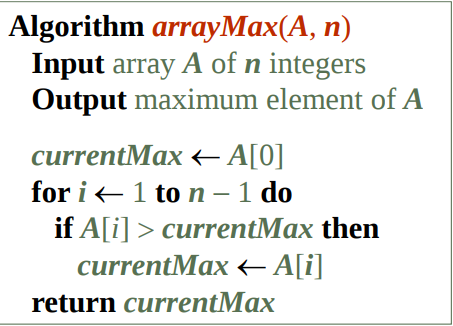
\includegraphics[scale=0.3]{Selection_001.png}}
\end{minipage}
\end{document}